\section*{20. Directed Graphs}\label{directed-graphs}

\subsection*{20.1 Introduction}\label{introduction:graphs}
Directed graphs are similar to undirected graphs, but there are arrows
between vertices instead of edges. Like undirected graphs, directed
graphs can be used to represent independence relations. They can also be
used as an alternative to counterfactuals to represent causal
relationships. Some people use the phrase \textbf{Bayesian network} to
refer to a directed graph endowed with a probability distribution. This
is a poor choice of terminology. Statistical inference for directed
graphs can be performed using frequentist or Bayesian methods so it is
misleading to call them Bayesian networks.

\subsection*{20.2 DAGs}\label{dags}
A \textbf{directed graph} \(\mathcal{G}\) consists of a set of vertices
\(V\) and an edge set \(E\) of ordered pairs of variables. If
\((X, Y) \in E\) then there is an arrow pointing from \(X\) to \(Y\).

\begin{python}
from graphviz import Digraph
d = Digraph()
d.edge('Y', 'X')
d.edge('Y', 'Z')
d
\end{python}

\begin{figure}[H]
\centering
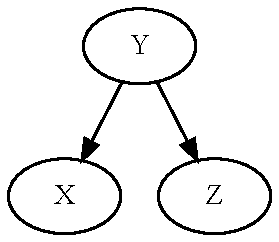
\includegraphics{Figure-20-01}
\end{figure}

If an arrow connects two variables \(X\) and \(Y\) (in either direction) we say that \(X\) and \(Y\) are \textbf{adjacent}. If there is an arrow from \(X\) to \(Y\) then \(X\) is a \textbf{parent} of \(Y\) and \(Y\) is a \textbf{child} of \(X\). The set of all parents of \(X\) is denoted by \(\pi_X\) or \(\pi(X)\). A \textbf{directed path} from \(X\) to \(Y\) is a set of vertices beginning with \(X\), ending with \(Y\) such that each pair is connected by an arrow and all of the arrows point in the same direction:
\[
X \rightarrow \cdots \rightarrow Y
\quad \text{or} \quad
X \leftarrow \cdots \leftarrow Y
\]
A sequence of adjacent vertices starting with \(X\) and ending with \(Y\) but ignoring the directions of the arrows is called an \textbf{undirected path}. \(X\) is an \textbf{ancestor} of \(Y\) if there is a directed path from \(X\) to \(Y\). We also say that \(Y\) is a \textbf{descendant} of \(X\).
A configuration of the form:
\[
X \rightarrow Y \leftarrow Z
\]
is called a \textbf{collider}. A configuration not of that form is called a \textbf{non-collider}, for example,
\[
X \rightarrow Y \rightarrow Z
\quad \text{or} \quad
X \leftarrow Y \leftarrow Z
\]
A directed path that starts and ends at the same variable is called a \textbf{cycle}. A directed graph is \textbf{acyclic} if it has no cycles. In this case we say that the graph is a \textbf{directed acyclic graph} or \textbf{DAG}. From now on, we will only deal with graphs that are DAGs.

\subsection*{20.3 Probability and DAGs}\label{probability:dags}
Let \(\mathcal{G}\) be a DAG with vertices \(V = (X_{1}, \dots, X_{k})\).
If \(\PROB\) is a distribution for \(V\) with probability function \(p\), we say that \textbf{\(\PROB\) is Markov to \(\mathcal{G}\)} or that \(M(\mathcal{G})\) represents \(\PROB\) if
\[
p(v) = \prod_{i=1}^{k} p(x_{i} | \pi_{i})
\]
where the \(\pi_{i}\) are the parents of \(X_{i}\). The set of distributions represented by \(\mathcal{G}\) is denoted by \(M(\mathcal{G})\).
The following Theorem says that \(\PROB \in M(\mathcal{G})\) if and only if the following \textbf{Markov Condition} holds. Roughly speaking, the Markov Condition says that every variable \(W\) is independent of the ``past'' given its parents.

\textbf{Theorem 20.3}. A distribution \(\PROB \in M(\mathcal{G})\) if and only if the following \textbf{Markov Condition} holds: for every variable \(W\),
\[
W \ci \bar{W} | \pi_W
\]
where \(\bar{W}\) denotes all the other variables except parents
and descendants of \(W\).

\subsection*{20.4 More Independence Relations}\label{more-independence-relations}
The Markov Condition allows us to list some independence relations.
These relations may logically imply other independence relations.
Consider this DAG:

\begin{python}
from graphviz import Digraph
d = Digraph()
d.edge('X2', 'X3')
d.edge('X1', 'X3')
d.edge('X1', 'X4')
d.edge('X3', 'X5')
d.edge('X4', 'X5')
d
\end{python}

\begin{figure}[H]
\centering
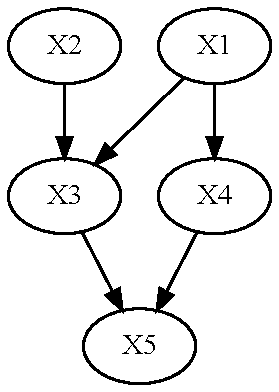
\includegraphics{Figure-20-02}
\end{figure}

The Markov Condition implies:
\begin{itemize}[tightlist]
\item
  \(X_{1} \ci X_{2}\)
\item
  \(X_{2} \ci \{ X_{1}, X_{4} \}\)
\item
  \(X_{3} \ci X_{4} | \{ X_{1}, X_{2} \}\)
\item
  \(X_{4} \ci \{ X_{2}, X_{3} \} | X_{1}\)
\item
  \(X_{5} \ci \{ X_{1}, X_{2} \} | \{X_{3}, X_{4}\}\)
\end{itemize}
It turns out that these conditions imply:
\[
\{ X_{4}, X_{5} \} \ci X_{2} | \{ X_{1}, X_{3} \}
\]
How do we find these extra independence relations? The answer is
\textbf{d-separation}, which can be summarized by 3 rules.
\textbf{The rules of d-separation}
\begin{enumerate}[tightlist,label={\arabic*.}]
\item
  In a non-collider \((X, Y, Z)\), \(X\) and \(Z\) are
  \textbf{d-connected}, but they are \textbf{d-separated} given \(Y\).
\item
  If \(X\) and \(Z\) collide at \(Y\) then \(X\) and \(Z\) are
  \textbf{d-separated} but they are \textbf{d-connected} given \(Y\).
\item
  Conditioning on the descendant of a collider has the same effect as
  conditioning on the collider. Thus in the figure below, \(X\) and
  \(Z\) are \textbf{d-separated} but they are \textbf{d-connected} given
  \(W\).
\end{enumerate}

\begin{python}
from graphviz import Digraph
d = Digraph()
d.edge('X', 'Y')
d.edge('Z', 'Y')
d.edge('Y', 'W')
d
\end{python}

\begin{figure}[H]
\centering
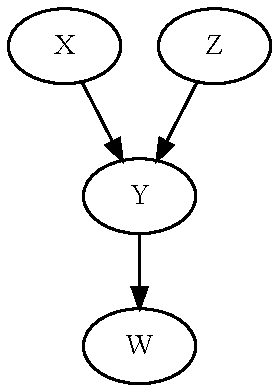
\includegraphics{Figure-20-03}
\end{figure}

Here is a more formal definition of d-separation. Let \(X\) and \(Y\) be
distinct vertices and let \(W\) be a set of vertices not containing
\(X\) or \(Y\). Then \(X\) and \(Y\) are \textbf{d-separated given
\(W\)} if there exists no undirected path \(U\) between \(X\) and \(Y\)
such that (i) every collider on \(U\) has a descendant in \(W\) and (ii)
no other vertex on \(U\) is in \(W\). If \(U\), \(V\), \(W\) are
distinct sets of vertices and \(U\) and \(V\) are not empty, then \(U\)
and \(V\) are d-separated given \(W\) if for every \(X \in U\) and
\(Y \in V\), \(X\) and \(Y\) are d-separated given \(W\). Vertices that
are not d-separated are said to be d-connected.

\textbf{Theorem 20.7 (Spirtes, Glymour and Scheines)}. Let \(A\), \(B\)
and \(C\) be disjoint sets of vertices. Then \(A \ci B | C\) if
and only if \(A\) and \(B\) are d-separated by \(C\).
Graphs that look different may imply the same independence relations. If
\(\mathcal{G}\) is a DAG, we let \(\mathcal{I}(\mathcal{G})\) denote all
the independence statements implied by \(\mathcal{G}\). Two DAGs
\(\mathcal{G}_{1}\) and \(\mathcal{G}_{2}\) for the same variables \(V\) are
\textbf{Markov equivalent} if
\(\mathcal{I}(\mathcal{G}_{1}) = \mathcal{I}(\mathcal{G}_{2})\). Given a DAG
\(\mathcal{G}\), let \(\text{skeleton}(\mathcal{G})\) denote the
undirected graph obtained by replacing the arrows with undirected edges.

\textbf{Theorem 20.9}. Two DAGs \(\mathcal{G}_{1}\) and \(\mathcal{G}_{2}\)
are Markov equivalent if and only if (i)
\(\text{skeleton}(\mathcal{G}_{1}) = \text{skeleton}(\mathcal{G}_{2})\) and
(ii) \(\mathcal{G}_{1}\) and \(\mathcal{G}_{2}\) have the same colliders.

\subsection*{20.5 Estimation for DAGs}\label{estimation-for-dags}
Let \(\mathcal{G}\) be a DAG. Assume that all variables
\(V = \{ X_{1}, \dots, X_m \}\) are discrete. The probability function can
be written
\[
p(v) = \prod_{i=1}^m p(x_{i} | \pi_{i})
\]
To estimate \(p(v)\) we need to estimate \(p(x_{i} | \pi_{i})\) for each
\(i\). Think of the parents of \(X_{i}\) as one discrete variable
\(\bar{X}_{i}\) with many levels. For example, suppose that \(X_{3}\)
has parents \(X_{1}\) and \(X_{2}\), and that \(X_{1} \in \{ 0, 1, 2 \}\)
while \(X_{2} \in \{ 0, 1 \}\). We can regard the parents \(X_{1}\) and
\(X_{2}\) as a single variable \(\bar{X}_{3}\) defined by
\[
\bar{X}_{3} = \begin{cases}
1 & \text{if } X_{1} = 0, X_{2} = 0\\
2 & \text{if } X_{1} = 0, X_{2} = 1\\
3 & \text{if } X_{1} = 1, X_{2} = 0\\
4 & \text{if } X_{1} = 1, X_{2} = 1\\
5 & \text{if } X_{1} = 2, X_{2} = 0\\
6 & \text{if } X_{1} = 2, X_{2} = 1\\
\end{cases}
\]
Hence we can write
\[
p(v) = \prod_{i=1}^m p(x_{i} | \bar{x}_{i})
\]

\textbf{Theorem 20.11}. Let \(V_{1}, \dots, V_{n}\) be IID random vectors
from distribution \(p\) where
\[
p(v) = \prod_{i=1}^{k} p(x_{i} | \bar{x}_{i})
\]
The maximum likelihood estimator of \(p\) is
\[
\hat{p}(v) = \prod_{i=1}^{k} \hat{p}(x_{i} | \bar{x}_{i})
\]
where
\[
\hat{p}(x_{i} | \bar{x}_{i}) = \frac{\# \{i : X_{i} = x_{i} \text{ and } \bar{X}_{i} = \bar{x}_{i} \}}{\# \{i : Y_{i} = y \}}
\]
It is possible to extend these ideas to continuous random variables as
well. For example, we might use some parametric model
\(p(x | \pi_x; \theta_x)\) for each conditional density. The likelihood
function is then
\[
\mathcal{L}(\theta) = \prod_{i=1}^{n} p(V_{i}; \theta) = \prod_{i=1}^{n} \prod_{j=1}^m p(X_{ij} | \pi_{j}; \theta_{j})
\]
where \(X_{ij}\) is the value of \(X_{j}\) for the \(i\)-th data point and
\(\theta_{j}\) are the parameters for the \(j\)-th conditional density. We
can then proceed using maximum likelihood.
So far, we have assumed that the structure of the DAG is given. One can
also try to estimate the structure of the DAG itself from the data.
However, there are many possible DAGs so you would need much data for
such a method to be reliable. Producing a valid, accurate confidence set
for the DAG structure would require astronomical sample sizes. DAGs are
thus most useful for encoding conditional independence information
rather than discovering it.

\subsection*{20.6 Causation Revisited}\label{causation-revisited}
We discussed causation in Chapter 19 using the idea of counterfactual
random variables. A different approach uses DAGs. The two approaches
are mathematically equivalent though they appear to be quite different.
The extra element in DAG is the idea of \textbf{intervention}.

\begin{python}
from graphviz import Digraph
d = Digraph()
d.edge('X', 'Y')
d.edge('Y', 'Z')
d.edge('X', 'Z')
d
\end{python}

\begin{figure}[H]
\centering
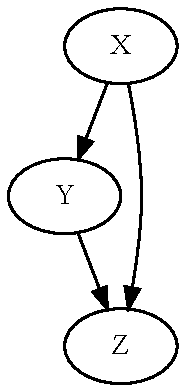
\includegraphics{Figure-20-04}
\end{figure}

Consider the DAG above. The probability function for a distribution
consistent with it has the form \(p(x, y, z) = p(x)p(y | x)p(z| x, y)\).
Here is pseudo-code for generating from this distribution:
\begin{console}
for i = 1, ..., n:
  x_i <- p_{X}(x_{i})
  y_i <- p_{Y | X}(y_{i} | x_{i})
  z_i <- p_{Z | X, Y}(z_{i} | x_{i}, y_{i})
\end{console}
Suppose we repeat this code many times yielding data
\((x_{1}, y_{1}, z_{1}), \dots, (x_{n}, y_{n}, z_{n})\). Among all the times that we
observe \(Y = y\), how often is \(Z = z\)? The answer to this question
is given by the conditional distribution of \(Z | Y\).
\begin{align*}
\PROB(Z = z | Y = y) &= \frac{\PROB(Y = y, Z = z)}{\PROB(Y = y)} = \frac{p(y, z)}{p(y)} \\
&= \frac{\sum_x p(x, y, z)}{p(y)} = \frac{\sum_x p(x) p(y | x) p(z | x, y)}{p(y)} \\
&= \sum_x p(z | x, y) \frac{p(y | x) p(x)}{p(y)} = \sum_x p(z | x, y) \frac{p(x, y)}{p(y)} \\
&= \sum_x p(z | x, y) p(x | y)
\end{align*}
Now suppose we \textbf{intervene} by changing the computer code.
Specifically, suppose we fix \(Y\) at the value \(y\). The code now
looks like this:
\begin{console}
set Y = y
for i = 1, ..., n:
  x_i <- p_{X}(x_{i})
  z_i <- p_{Z | X, Y}(z_{i} | x_{i}, y)
\end{console}
Having \textbf{set} \(Y = y\), how often was \(Z = z\)? To answer, note
that the intervention has changed the joint probability to be
\[
p^{*}(x, z) = p(x) p(z | x, y)
\]
The answer to our question is given by the marginal distribution
\[
p^{*}(z) = \sum_x p^{*}(x, z) = \sum_x p(x) p(z | x, y)
\]
We shall denote this as \(\PROB(Z = z | Y := y)\) or
\(p(z | Y := y)\). We call \(\PROB(Z = z | Y = y)\)
\textbf{conditioning by observation} or \textbf{passive conditioning}.
We call \(\PROB(Z = z | Y := y)\) \textbf{conditioning by
intervention} or \textbf{active conditioning}.
\begin{itemize}[tightlist]
\item
  Passive conditioning is used to answer a predictive question like
  ``Given that Joe smokes, what is the probability that he will get lung
  cancer?''.
\item
  Active conditioning is used to answer a predictive question like ``If
  Joe quits smoking, what is the probability that he will get lung
  cancer?''.
\end{itemize}
Consider a pair \((\mathcal{G}, \PROB)\) where \(\mathcal{G}\) is a
DAG and \(\PROB\) is a distribution for the variables \(V\) of the
DAG. Let \(p\) denote the probability function for \(p\). Consider
intervening and fixing a variable \(X\) to be equal to \(x\). We
represent the intervention by doing two things:
\begin{enumerate}[tightlist,label={\arabic*.}]
\item
  Create a new DAG \(\mathcal{G}^{*}\) by removing all arrows pointing
  into \(X\);
\item
  Create a new distribution \(\PROB^{*}\) with probability function
  \(p^{*}(v) = \PROB(V = v | X := x)\) by removing the term
  \(p(x | \pi_X)\) from \(p(v)\).
\end{enumerate}
The new pair \((\mathcal{G}^{*}, \PROB^{*})\) represents the
intervention ``set \(X = x\)''.
We can use DAGs to represent confounding variables. If \(X\) is a
treatment and \(Y\) is an outcome, a confounding variable \(Z\) is a
variable with arrows into both \(X\) and \(Y\). It is easy to check,
using the formalism of interventions, that the following facts are true.
\begin{itemize}[tightlist]
\item
  In a randomized study, the arrow between \(Z\) and \(X\) is broken. In
  this case, even with \(Z\) unobserved, the causal relationship between
  \(X\) and \(Y\) is estimable because it can be shown that
  \(\EXP(Y | X := x) = \EXP(Y | X = x)\) which does not
  involved the unobserved \(Z\).\\
\item
  In an observational study, with all confounders observed, we again get
  \(\EXP(Y | X := x) = \int \EXP(Y | X = x, Z = z) d F_Z(z)\)
  as a formula for the expectation. if \(Z\) is unobserved then we
  cannot estimate the causal effect because this expectation involves
  the unobserved \(Z\).
  \(\PROB(Y = y | X = x) \neq \PROB(Y = y | X := x)\) which is
  just another way of saying that causation is not association.
\end{itemize}
In fact, we can make a precise connection between DAGs and
counterfactuals as follows. Suppose that \(X\) and \(Y\) are binary.
Define the confounding variable \(Z\) by
\[
Z = \begin{cases}
1 & \text{if } (C_{0}, C_{1}) = (0, 0) \\
2 & \text{if } (C_{0}, C_{1}) = (0, 1) \\
3 & \text{if } (C_{0}, C_{1}) = (1, 0) \\
4 & \text{if } (C_{0}, C_{1}) = (1, 1)
\end{cases}
\]
From this approach, one can make the correspondence between the DAG and
counterfactual approaches explicit. This is left as an exercise for the
reader.

\subsection*{20.8 Exercises}

\textbf{Exercise 20.8.1}. Consider the three DAGs below without a
collider. Prove that \(X \ci Z | Y\).

\begin{python}
from graphviz import Digraph
a = Digraph()
a.edge('X', 'Y')
a.edge('Y', 'Z')
a
\end{python}

\begin{figure}[H]
\centering
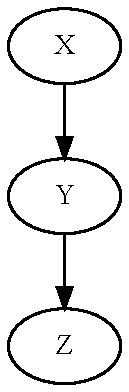
\includegraphics{Figure-20-05}
\end{figure}


\begin{python}
from graphviz import Digraph
b = Digraph()
b.edge('Y', 'X')
b.edge('Z', 'Y')
b
\end{python}

\begin{figure}[H]
\centering
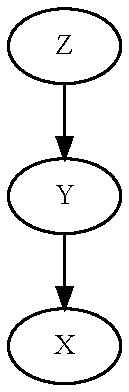
\includegraphics{Figure-20-06}
\end{figure}


\begin{python}
from graphviz import Digraph
c = Digraph()
c.edge('Y', 'X')
c.edge('Y', 'Z')
c
\end{python}

\begin{figure}[H]
\centering
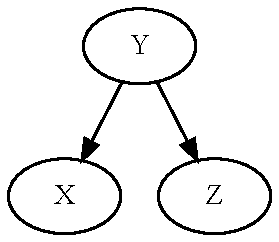
\includegraphics{Figure-20-07}
\end{figure}


\textbf{Solution}.
Note that for all three graphs \(X\) and \(Z\) are d-separated by \(Y\)
-- the only undirected path \((X, Y, Z)\) has no colliders, and all its
vertices other than \(X\) and \(Z\) (i.e.~\(\{ Y \}\)) are listed in the
d-separation condition. Thus, conditions (i) and (ii) on the definition
of d-separation holds.
Therefore, from Theorem 20.7, \(X \ci Z | Y\).

\textbf{Exercise 20.8.2}. Consider the DAG below. Prove that
\(X \ci Z\) and that \(X\) and \(Y\) are dependent given \(Y\).

\begin{python}
from graphviz import Digraph
d = Digraph()
d.edge('Y', 'X')
d.edge('Y', 'Z')
d
\end{python}

\begin{figure}[H]
\centering
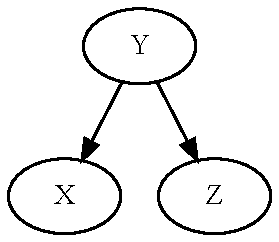
\includegraphics{Figure-20-08}
\end{figure}

\textbf{Solution}.
Note that \(X\) and \(Z\) are d-connected by \(Y\) -- the undirected
path \((X, Y, Z)\) has one collider containing \(Y\), so the definition
of d-separation does not hold. Therefore, from Theorem 20.7, \(X\) and
\(Z\) are dependent given \(Y\).
On the other hand, note that \(X\) and \(Z\) are d-separated given the
empty set -- the only path from \(X\) to \(Z\) goes through \(Y\), which
is not in the empty set. Thus, from Theorem 20.7, \(X \ci Z\).

\textbf{Exercise 20.8.3}. Let \(X \in \{0, 1\}\), \(Y \in \{0, 1\}\),
\(Z \in \{ 0, 1, 2 \}\). Suppose the distribution of \((X, Y, Z)\) is
Markov to:
\[
X \longrightarrow Y \longrightarrow Z
\]
Create a joint distribution \(p(x, y, z)\) that is Markov to this DAG.
Generate 1000 random vectors from this distribution. Estimate the
distribution from the data using maximum likelihood. Compare the
estimated distribution to the true distribution. Let
\(\theta = (\theta_{000}, \theta_{001}, \dots, \theta_{112})\) where
\(\theta_{rst} = \PROB(X = r, Y = s, Z = t)\). Use the bootstrap to
get the standard errors and 95\% confidence interval for these 12
parameters.

\textbf{Solution}. Create the following distributions:
\begin{align*}
p_{X}(x) & = 
\begin{cases}
1/2 & \text{if } x \in \{0, 1\} \\
0 & \text{otherwise}
\end{cases}
\\
p_{Y | X}(y | x) & = 
\begin{cases}
3/4 & \text{if } y = x \\
1/4 & \text{if } x + y = 1 \\
0 & \text{otherwise}
\end{cases}
\\
p_{Z | Y}(z | y) & = 
\begin{cases}
1/2 &\text{if } z = y \text{ and } z \in \{ 0, 1, 2 \}\\
1/4 &\text{if } z \neq y \text{ and } z \in \{ 0, 1, 2 \} \\
0 &\text{otherwise}
\end{cases}
\end{align*}
and a joint distribution
\[
p(x, y, z) = p_{X}(x) p_{Y | X}(y | x) p_{Z | Y}(z | y)
\]
By construction, this distribution is Markov to the given DAG.
More explicitly, the joint probability distribution is:
\[
\begin{array}{ccc|c}
X & Y & Z & p \\
\hline
0 & 0 & 0 & .18750 \\
0 & 0 & 1 & .09375 \\
0 & 0 & 2 & .09375 \\
0 & 1 & 0 & .03125 \\
0 & 1 & 1 & .06250 \\
0 & 1 & 2 & .03125 \\
1 & 0 & 0 & .06250 \\
1 & 0 & 1 & .03125 \\
1 & 0 & 2 & .03125 \\
1 & 1 & 0 & .09375 \\
1 & 1 & 1 & .18750 \\
1 & 1 & 2 & .09375 \\
\end{array}
\]
The maximum likelihood estimator of \(p\) is
\[
\hat{p}(v) = \prod_{i=1}^{k} \hat{p}(x_{i} | \bar{x}_{i})
\]
where
\[
\hat{p}(x_{i} | \bar{x}_{i}) = \frac{\# \{i : X_{i} = x_{i} \text{ and } \bar{X}_{i} = \bar{x}_{i} \}}{\# \{i : Y_{i} = y \}}
\]

\begin{python}
import numpy as np
def generate_samples(n):
    seeds = np.random.uniform(low=0, high=1, size=(n, 3))
    result = np.zeros((n, 3), dtype=int)
    result[:, 0] = seeds[:, 0] < 1/2
    result[:, 1] = np.where(seeds[:, 1] < 3/4, 
    result[:, 0], 1 - result[:, 0])
    result[:, 2] = np.where(seeds[:, 2] < 1/2, 
    result[:, 1], (result[:, 1] + np.where(seeds[:, 2] < 3/4, 1, 2)) % 3)
    return result
def estimate_parameters(X):
    n = X.shape[0]
    
    p_hat_x0 = np.sum(X[:, 0] == 0) / n
    p_hat_x1 = np.sum(X[:, 0] == 1) / n
    
    p_hat_y0_x0 = np.sum((X[:, 0] == 0) & (X[:, 1] == 0)) / np.sum(X[:, 0] == 0)
    p_hat_y1_x0 = np.sum((X[:, 0] == 0) & (X[:, 1] == 1)) / np.sum(X[:, 0] == 0)
    
    p_hat_y0_x1 = np.sum((X[:, 0] == 1) & (X[:, 1] == 0)) / np.sum(X[:, 0] == 1)
    p_hat_y1_x1 = np.sum((X[:, 0] == 1) & (X[:, 1] == 1)) / np.sum(X[:, 0] == 1)
    
    p_hat_z0_y0 = np.sum((X[:, 2] == 0) & (X[:, 1] == 0)) / np.sum(X[:, 1] == 0)
    p_hat_z1_y0 = np.sum((X[:, 2] == 1) & (X[:, 1] == 0)) / np.sum(X[:, 1] == 0)
    p_hat_z2_y0 = np.sum((X[:, 2] == 2) & (X[:, 1] == 0)) / np.sum(X[:, 1] == 0)
    p_hat_z0_y1 = np.sum((X[:, 2] == 0) & (X[:, 1] == 1)) / np.sum(X[:, 1] == 1)
    p_hat_z1_y1 = np.sum((X[:, 2] == 1) & (X[:, 1] == 1)) / np.sum(X[:, 1] == 1)
    p_hat_z2_y1 = np.sum((X[:, 2] == 2) & (X[:, 1] == 1)) / np.sum(X[:, 1] == 1)
    
    theta_hat = np.array([
        p_hat_x0 * p_hat_y0_x0 * p_hat_z0_y0,
        p_hat_x0 * p_hat_y0_x0 * p_hat_z1_y0,
        p_hat_x0 * p_hat_y0_x0 * p_hat_z2_y0,
        
        p_hat_x0 * p_hat_y1_x0 * p_hat_z0_y1,
        p_hat_x0 * p_hat_y1_x0 * p_hat_z1_y1,
        p_hat_x0 * p_hat_y1_x0 * p_hat_z2_y1,
        
        p_hat_x1 * p_hat_y0_x1 * p_hat_z0_y0,
        p_hat_x1 * p_hat_y0_x1 * p_hat_z1_y0,
        p_hat_x1 * p_hat_y0_x1 * p_hat_z2_y0,
        
        p_hat_x1 * p_hat_y1_x1 * p_hat_z0_y1,
        p_hat_x1 * p_hat_y1_x1 * p_hat_z1_y1,
        p_hat_x1 * p_hat_y1_x1 * p_hat_z2_y1
    ])
    
    return theta_hat
true_distribution = np.array([
    0.5 * 0.75 * 0.5,
    0.5 * 0.75 * 0.25,
    0.5 * 0.75 * 0.25,
    0.5 * 0.25 * 0.25,
    0.5 * 0.25 * 0.5,
    0.5 * 0.25 * 0.25,
    0.5 * 0.25 * 0.5,
    0.5 * 0.25 * 0.25,
    0.5 * 0.25 * 0.25,
    0.5 * 0.75 * 0.25,
    0.5 * 0.75 * 0.5,
    0.5 * 0.75 * 0.25
])
\end{python}

\begin{python}
n = 1000
X = generate_samples(n)
\end{python}

\begin{python}
theta_hat = estimate_parameters(X)
\end{python}

\begin{python}
import matplotlib.pyplot as plt
import seaborn as sns
sns.set()
ind = np.arange(12)
labels = ['000', '001', '002', '010', '011', '012', '100', '101', '102', '110', '111', '112']
x = np.arange(len(labels))
fig, ax = plt.subplots(figsize=(12, 8))
ax.plot(x, theta_hat, label='Estimated', 
        linestyle='', marker='+', ms=10)
ax.plot(x, true_distribution, label='Actual', 
        linestyle='', marker='x', ms=10)
ax.set_title('Estimated vs actual parameters')
ax.set_xticks(x)
ax.set_xticklabels(labels)
ax.legend()
fig.tight_layout()
plt.show();
\end{python}


\setkeys{Gin}{height=0.40\textheight}

\begin{figure}[H]
\centering
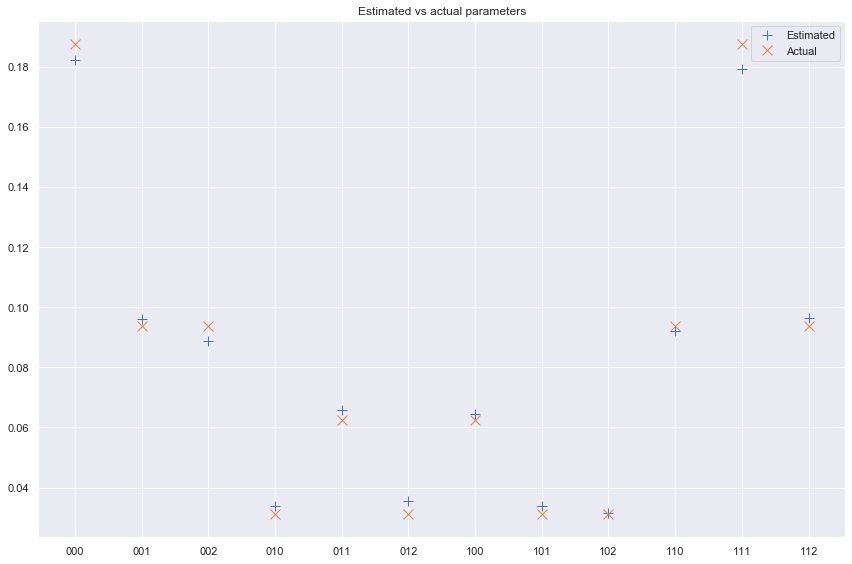
\includegraphics{Figure-20-09}
\end{figure}


\begin{python}
# Bootstrapping:
from tqdm import tqdm_notebook
B = 10000
parameters_bootstrap = np.empty((B, 12))
for i in tqdm_notebook(range(B)):
    XX = generate_samples(n)
    parameters_bootstrap[i] = estimate_parameters(XX)
    
se_theta_hat = parameters_bootstrap.std(axis=0)
theta_p05 = np.quantile(parameters_bootstrap, 0.05, axis=0)
theta_p95 = np.quantile(parameters_bootstrap, 0.95, axis=0)
\end{python}

\begin{python}
import matplotlib.pyplot as plt
import seaborn as sns
sns.set()
ind = np.arange(12)
labels = ['000', '001', '002', '010', '011', '012', '100', '101', '102', '110', '111', '112']
x = np.arange(len(labels))
fig, ax = plt.subplots(figsize=(12, 8))
ax.plot(x, theta_hat, label='Estimated', linestyle='', marker='+', ms=10)
ax.plot(x, true_distribution, label='Actual', linestyle='', marker='x', ms=10)
ax.plot(x, theta_p95, label='95% percentile', linestyle='', marker='_', ms=10)
ax.plot(x, theta_p05, label='5% percentile', linestyle='', marker='_', ms=10)
ax.plot(x, theta_hat - 2*se_theta_hat, label='Estimated - 2 SE', linestyle='', marker='1', ms=10)
ax.plot(x, theta_hat + 2*se_theta_hat, label='Estimated + 2 SE', linestyle='', marker='2', ms=10)
ax.set_title('Estimated vs actual parameters (with confidence + SE bounds)')
ax.set_xticks(x)
ax.set_xticklabels(labels)
ax.legend()
fig.tight_layout()
plt.show();
\end{python}

\begin{figure}[H]
\centering
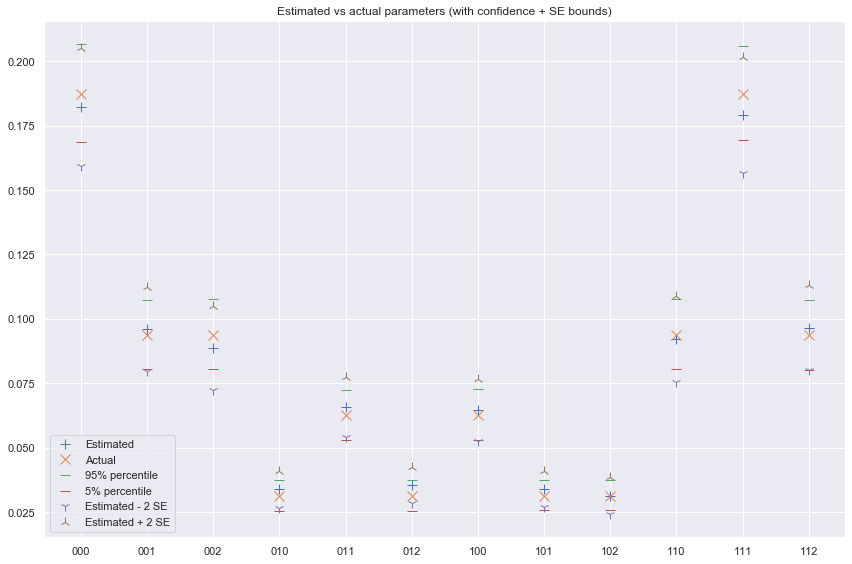
\includegraphics{Figure-20-10}
\end{figure}


\textbf{Exercise 20.8.4}. Let \(V = (X, Y, Z)\) have the joint
distribution
\begin{align*}
X &\sim \text{Bernoulli}\left(\frac{1}{2}\right) \\
Y | X = x &\sim \text{Bernoulli}\left(\frac{e^{4x - 2}}{1 + e^{4x - 2}}\right) \\
Z | X = x, Y = y &\sim \text{Bernoulli}\left(\frac{e^{2(x+y)-2}}{1 + e^{2(x+y)-2}}\right)
\end{align*}
\textbf{(a)} Find an expression for \(\PROB(Z = z | Y = y)\). In
particular, find \(\PROB(Z = 1 | Y = 1)\).
\textbf{(b)} Write a program to simulate the model. Conduct a simulation
and compute \(\PROB(Z = 1 | Y = 1)\) empirically. Plot this as a
function of the simulation size \(N\). It should converge to the
theoretical value you computed in (a).
\textbf{(c)} Write down an expression for
\(\PROB(Z = 1 | Y := y)\). In particular, find
\(\PROB(Z = 1 | Y := 1)\).
\textbf{(d)} Modify your program to simulate the intervention ``set
\(Y = 1\)''. Conduct a simulation and compute
\(\PROB(Z = 1 | Y := 1)\) empirically. Plot this as a function of
the simulation size \(N\). It should converge to the theoretical value
you computed in (c).

\textbf{Solution}.
\textbf{(a)}
We have:
\begin{align*}
\PROB(Z = z | Y = y) &= \frac{\PROB(Y = y, Z = z)}{\PROB(Y = y)} = \frac{p(y, z)}{p(y)} \\
&= \frac{\sum_x p(x, y, z)}{p(y)} = \frac{\sum_x p(x) p(y | x) p(z | x, y)}{p(y)} \\
&= \sum_x p(z | x, y) \frac{p(y | x) p(x)}{p(y)} = \sum_x p(z | x, y) \frac{p(x, y)}{p(y)} \\
&= \sum_x p(z | x, y) p(x | y)
\end{align*}
Let \(\alpha = \frac{e^{-2}}{1 + e^{-2}}\). Note that
\(\frac{e^{-2}}{1 + e^{-2}} + \frac{e^{2}}{1 + e^{2}} = 1\), so
\(1 - \alpha = \frac{e^{2}}{1 + e^{2}}\).
Looking explicitly at each potential outcome for the joint distribution
of \(X\) and \(Y\), we get:
\[
\begin{array}{c | cc | c}
p(x, y) & Y = 0 & Y = 1 & \\
\hline
X = 0 & (1 - \alpha) / 2 & \alpha / 2 & 1/2 \\
X = 1 & \alpha / 2 & (1 - \alpha) / 2 & 1/2 \\
\hline
  & 1/2 & 1/2 & 1
\end{array}
\]
Therefore,
\[
X | Y = 0 \sim \text{Bernoulli}\left( \alpha \right) 
\quad \text{and} \quad
X | Y = 1 \sim \text{Bernoulli}\left( 1 - \alpha \right) 
\]
or, more generally,
\[
X | Y = y \sim \text{Bernoulli}\left( \frac{e^{4y - 2}}{1 + e^{4y - 2}} \right) 
\]
Then, for \(Z = 1\) and \(y \in \{ 0, 1 \}\),
\begin{align*}
\PROB(Z = 1 | Y = y) &= \sum_x p(z = 1 | x, y) p(x | y) \\
&= p(z = 1 | x = 0, y) p(x = 0 | y) + p(z = 1 | x = 1, y) p(x = 1 | y) \\
&= \frac{e^{2y - 2}}{1 + e^{2y - 2}} \left( 1 - \frac{e^{4y - 2}}{1 + e^{4y - 2}} \right) + \frac{e^{4y - 2}}{1 + e^{4y - 2}} \frac{e^{4y - 2}}{1 + e^{4y - 2}}
\end{align*}
Explicitly,
\begin{align*}
\PROB(Z = 1 | Y = 0) &= \alpha (1 - \alpha) + \alpha^{2} \\
&= \alpha  &\approx 0.1192 \\
\PROB(Z = 0 | Y = 0) &= 1 - \PROB(Z = 1 | Y = 0) \\
&= 1 - \alpha &\approx 0.8808\\
\PROB(Z = 1 | Y = 1) &= \frac{1}{2} \alpha + (1 - \alpha)^{2} &\approx 0.8354\\
\PROB(Z = 0 | Y = 1) &= 1 - \PROB(Z = 1 | Y = 1) \\
&= 1 - \left(\frac{1}{2} \alpha + (1 - \alpha)^{2} \right) &\approx 0.1646\\
\end{align*}
\textbf{(b)}

\begin{python}
import numpy as np
def generate_samples(n):
    seeds = np.random.uniform(low=0, high=1, size=(n, 3))
    
    x = np.where(seeds[:, 0] < 1/2, 1, 0)
    y = np.where(seeds[:, 1] < np.exp(4*x - 2) / (1 + np.exp(4*x - 2)), 1, 0)
    z = np.where(seeds[:, 2] < np.exp(2*(x + y) - 2) / (1 + np.exp(2*(x + y) - 2)), 1, 0)
    
    result = np.zeros((n, 3), dtype=int)
    result[:, 0] = x
    result[:, 1] = y
    result[:, 2] = z
    
    return result
def estimate_z_given_y(X, z, y):
    # Just estimate 0.5 if there are no valid samples
    if np.sum((X[:, 1] == y)) == 0:
        return 0.5
    return np.sum((X[:, 1] == y) & (X[:, 2] == z)) / np.sum((X[:, 1] == y))
\end{python}

\begin{python}
# Generate data
X = generate_samples(10**6)
\end{python}

\begin{python}
# Estimate with various segments of the data
n_values = np.floor(np.logspace(0, 6, base=10)).astype(int)
z_estimates = [estimate_z_given_y(X[:k], 1, 1) for k in n_values]
\end{python}

\begin{python}
# Plot estimates
import matplotlib.pyplot as plt
plt.figure(figsize=(12, 8))
plt.scatter(n_values, z_estimates)
plt.xscale('log')
plt.xlabel('N')
plt.ylabel('Z | Y = 1')
plt.title('Empirical estimates of Z | Y = 1')
plt.show()
\end{python}

\begin{figure}[H]
\centering
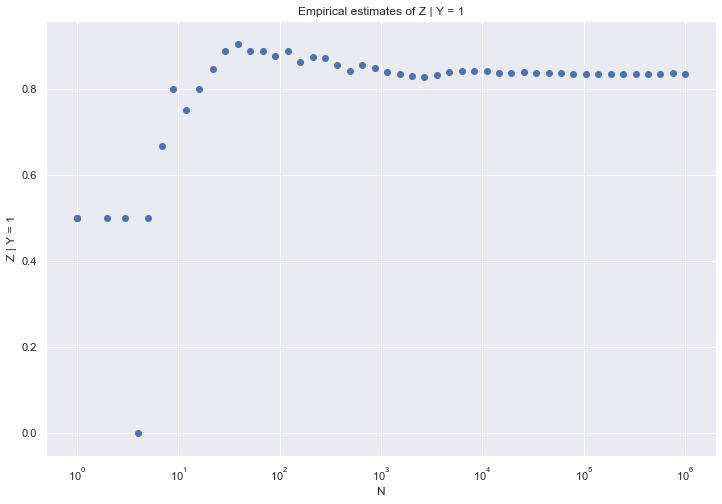
\includegraphics{Figure-20-11}
\end{figure}

\textbf{(c)}
Fixing \(Y := y \in \{0, 1\}\), we get:
\begin{align*}
\PROB(Z = 1 | Y := y) &= p^{*}(z = 1) = \sum_x p^{*}(x, z = 1) = \sum_x p(x) p(z = 1 | x, y) \\
&= \frac{1}{2} \frac{e^{2y-2}}{1 + e^{2y-2}} + \frac{1}{2} \frac{e^{2y}}{1 + e^{2y}}
\end{align*}
Explicitly,
\begin{align*}
\PROB(Z = 1 | Y := 0) &= \frac{1}{2} \alpha + \frac{1}{2}\frac{1}{2} \\
&= \frac{1}{4} + \frac{\alpha}{2} &\approx 0.3096 \\
\PROB(Z = 0 | Y := 0) &= 1 - \PROB(Z = 1 | Y := 0) \\
&= \frac{3}{4} - \frac{\alpha}{2} &\approx 0.6904 \\
\PROB(Z = 1 | Y := 1) &= \frac{1}{2} \frac{1}{2} + \frac{1}{2} \left( 1 - \alpha \right) \\
&= \frac{3}{4} - \frac{\alpha}{2} &\approx 0.6904 \\
\PROB(Z = 0 | Y := 1) &= 1 - \PROB(Z = 1 | Y := 1) \\
&= \frac{1}{4} + \frac{\alpha}{2} &\approx 0.3096
\end{align*}
\textbf{(d)}

\begin{python}
import numpy as np
def generate_samples_modified(n, y0):
    seeds = np.random.uniform(low=0, high=1, size=(n, 3))
    
    x = np.where(seeds[:, 0] < 1/2, 1, 0)
    y = y0 * np.ones(n, dtype=int)
    z = np.where(seeds[:, 2] < np.exp(2*(x + y) - 2) / (1 + np.exp(2*(x + y) - 2)), 1, 0)
    
    result = np.zeros((n, 3), dtype=int)
    result[:, 0] = x
    result[:, 1] = y
    result[:, 2] = z
    
    return result
\end{python}

\begin{python}
# Generate data
Xd = generate_samples_modified(n=10**6, y0=1)
\end{python}

\begin{python}
# Estimate with various segments of the data
n_values = np.floor(np.logspace(0, 6, base=10)).astype(int)
zd_estimates = [estimate_z_given_y(Xd[:k], 1, 1) for k in n_values]
\end{python}

\begin{python}
# Plot estimates
import matplotlib.pyplot as plt
plt.figure(figsize=(12, 8))
plt.scatter(n_values, zd_estimates)
plt.xscale('log')
plt.xlabel('N')
plt.ylabel('Z | Y := 1')
plt.title('Empirical estimates of Z | Y := 1')
plt.show()
\end{python}

\begin{figure}[H]
\centering
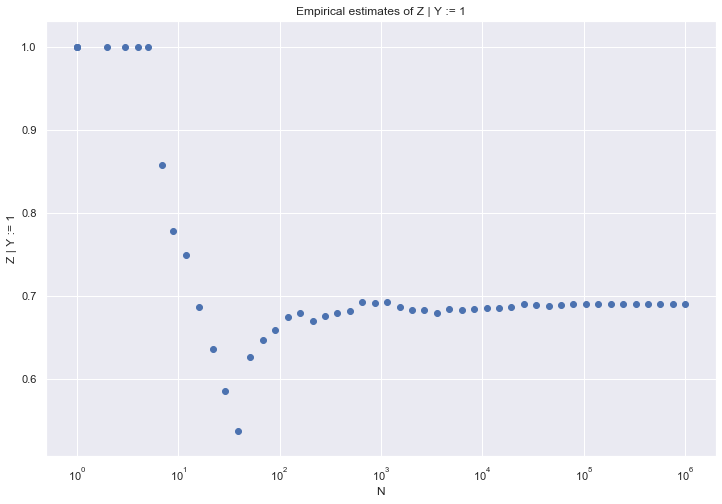
\includegraphics{Figure-20-12}
\end{figure}


\textbf{Exercise 20.8.5}. This is a continuous, Gaussian version of the
last question. Let \(V = (X, Y, Z)\) have the following joint
distribution:
\begin{align*}
X &\sim \text{Normal}(0, 1) \\
Y | X = x &\sim \text{Normal}(\alpha x, 1) \\
Z | X = x, Y = y &\sim \text{Normal}(\beta y + \gamma x, 1)
\end{align*}
Here, \(\alpha\), \(\beta\) and \(\gamma\) are fixed parameters.
Economists refer to models like this as \emph{structural equation
models}.
\textbf{(a)} Find an explicit expression for \(f(z | y)\) and
\(\EXP(Z | Y = y) = \int z f(z | y) dz\).
\textbf{(b)} Find an explicit expression for \(f(z | Y := y)\) and then
find \(\EXP(Z | Y := y) \equiv \int z f(z | Y := y) dy\). Compare
to (b).
\textbf{(c)} Find the joint distribution of \((Y, Z)\). Find the
correlation \(\rho\) between \(Y\) and \(Z\).
\textbf{(d)} Suppose that \(X\) is not observed and we try to make
causal conclusions from the marginal distribution of \((Y, Z)\). (Think
of \(X\) as unobserved confounding variables.) In particular, suppose we
declare that \(Y\) causes \(Z\) if \(\rho \neq 0\) and we declare that
\(Y\) does not cause \(Z\) if \(\rho = 0\). Show that this will lead to
erroneous conclusions.
\textbf{(e)} Suppose we conduct a randomized experiment in which \(Y\)
is randomly assigned. To be concrete, suppose that
\begin{align*}
X &\sim \text{Normal}(0, 1) \\
Y | X = x &\sim \text{Normal}(\alpha, 1) \\
Z | X = x, Y = y &\sim \text{Normal}(\beta y + \gamma x, 1)
\end{align*}
Show that the method in (d) now yields correct conclusions
i.e.~\(\rho = 0\) if and only if \(f(z | Y := y)\) does not depend on
\(y\).

\textbf{Solution}.
\textbf{(a)}
The joint distribution of \(X\) and \(Y\) is:
\begin{align*}
f_{X, Y}(x, y) &= f_X(x) f_{Y | X}(y | x) \\
&= \left(\frac{1}{\sigma_X \sqrt{2\pi}} \exp \left\{-\frac{1}{2} \left(\frac{x - \mu_X}{\sigma_X}\right)^{2} \right\} \right)
\left(\frac{1}{\sigma_{Y | X} \sqrt{2\pi}} \exp \left\{-\frac{1}{2} \left(\frac{y - \mu_{Y | X}}{\sigma_{Y | X}}\right)^{2} \right\}\right) \\
&= \left(\frac{1}{\sqrt{2\pi}}\right)^{2} \exp \left\{ -\frac{1}{2} \left( x^{2} + (y - \alpha x)^{2}\right) \right\} \\
&= (2 \pi)^{-2 / 2} \det (\Sigma_{X, Y})^{-1/2} \exp \left\{ -\frac{1}{2} (v - \mu_{X, Y})^T \Sigma_{X, Y}^{-1} (v - \mu_{X, Y})\right\}
\end{align*}
where
\[
v = \begin{bmatrix}x \\ y\end{bmatrix},
\quad \mu_{X, Y} = \begin{bmatrix}0 \\ 0\end{bmatrix}
\quad \text{and} \quad
\Sigma_{X, Y} = \begin{bmatrix}
1 & \alpha \\
\alpha & 1 + \alpha^{2}
\end{bmatrix}
\]
or, in words, the joint distribution of \(X, Y\) is a multivariate
normal with mean \(\mu_{X, Y} = 0\) and variance \(\Sigma_{X, Y}\).
\[
(X, Y) \sim \text{Normal}( 0, \Sigma_{X, Y})
\]
This can be obtained by inspection, by defining the inverse variance
matrix
\[
\Sigma_{X, Y}^{-1} = \begin{bmatrix}
1 + \alpha^{2} & -\alpha \\
-\alpha      & 1
\end{bmatrix}
\]
from expanding \(x^{2} + (y - \alpha x)^{2}\) and
\((v - \mu_{X, Y})^T \Sigma_{X, Y}^{-1} (v - \mu_{X, Y})\), taking mean
\(\mu_{X, Y} = 0\) assuming the inverse matrix is symmetric, and
equating the coefficients for the monomials \(x^{2}, y^{2}, xy\).
The joint distribution of \(X, Y, Z\) then is:
\begin{align*}
f_{X, Y, Z} (x, y, z) &= f_{X, Y}(x, y) f_{Z | X, Y}(z | x, y) \\
&= \left(\frac{1}{\sqrt{2\pi}}\right)^{2} \exp \left\{ -\frac{1}{2} \left( x^{2} + (y - \alpha x)^{2}\right) \right\} 
\left(\frac{1}{\sqrt{2\pi}} \right) \exp \left\{ -\frac{1}{2} (z - (\beta y + \gamma x))^{2}\right\} \\
&= \left(\frac{1}{\sqrt{2\pi}}\right)^{3} \exp \left\{ -\frac{1}{2} \left( x^{2} + (y - \alpha x)^{2} + (z - (\beta y + \gamma x))^{2}\ \right) \right\} \\
&= (2\pi)^{-3/2} \det(\Sigma_{X, Y, Z})^{-1/2} \exp \left\{ -\frac{1}{2} (v - \mu_{X, Y, Z})^T \Sigma_{X, Y, Z}^{-1} (v - \mu_{X, Y, Z})\right\}
\end{align*}
where
\[
v = 
\begin{bmatrix}
x \\ y \\ z
\end{bmatrix},
\quad \mu_{X, Y, Z} = 
\begin{bmatrix}
0 \\ 0 \\ 0
\end{bmatrix}
\]
and
\[
\Sigma_{X, Y, Z} = \begin{bmatrix}
1 & \alpha & \alpha \beta + \gamma\\
\alpha & 1 + \alpha^{2} & \alpha(\alpha \beta + \gamma) + \beta \\
\alpha \beta + \gamma & \alpha(\alpha \beta + \gamma) + \beta & -(\alpha - \beta\gamma)^{2} + (\beta^{2} + 1)(\alpha^{2} + \gamma^{2} + 1)
\end{bmatrix}
\]
or, in words, the joint distribution of \(X, Y, Z\) is a multivariate
normal with mean \(\mu_{X, Y, Z} = 0\) and variance
\(\Sigma_{X, Y, Z}\).
\[
(X, Y, Z) \sim \text{Normal}(0, \Sigma_{X, Y, Z})
\]
This can be obtained by inspection, by defining the inverse variance
matrix
\[
\Sigma_{X, Y, Z}^{-1} = \begin{bmatrix}
1 + \alpha^{2} + \gamma^{2} & -\alpha + \beta \gamma & -\gamma \\
-\alpha + \beta \gamma  & 1 + \beta^{2}            & -\beta  \\
-\gamma                 & -\beta                 & 1
\end{bmatrix}
\]
from expanding \(x^{2} + (y - \alpha x)^{2} + (z - (\beta y + \gamma x))^{2}\)
and \((v - \mu_{X, Y, Z})^T \Sigma_{X, Y, Z}^{-1} (v - \mu_{X, Y, Z})\),
taking mean \(\mu_{X, Y, Z} = 0\), assuming the inverse matrix is
symmetric, and equating the coefficients for the monomials
\(x^{2}, y^{2}, z^{2}, xy, xz, yz\). A symbolic mathematics library was then
used to calculate the inverse and simplify it as above.
Now that we have characterized the joint distribution of \(X, Y, Z\), we
can use Theorem 15.5 to first compute the marginal distribution of
\(Y, Z\), and then use it again to compute the conditional distribution
of \(Z | Y = y\).
The marginal distribution of \(Y, Z\) is
\[
(Y, Z) \sim \text{Normal}(0, \Sigma_{Y, Z})
\]
where
\[
\Sigma_{Y, Z} = 
\begin{bmatrix}
1 + \alpha^{2} & \alpha(\alpha \beta + \gamma) + \beta \\
\alpha(\alpha \beta + \gamma) + \beta & -(\alpha - \beta\gamma)^{2} + (\beta^{2} + 1)(\alpha^{2} + \gamma^{2} + 1)
\end{bmatrix}
\]
Now, the conditional distribution of \(Z | Y = y\) is:
\[
Z | Y = y \sim \text{Normal}(\mu_{Z | Y} (y), \Sigma_{Z | Y}(y))
\]
where
\begin{align*}
\mu_{Z | Y}(y) 
& = \mu_Z + \Sigma_{zy} \Sigma_{yy}^{-1} (y - \mu_y) = \frac{\alpha(\alpha \beta + \gamma) + \beta}{\alpha^{2} + 1} y
\\
\Sigma_{Z | Y}(y) 
& = \Sigma_{zz} - \Sigma_{zy} \Sigma_{yy}^{-1} \Sigma_{yz} = \frac{\alpha^{2} + \gamma^{2} + 1}{\alpha^{2} + 1}
\end{align*}
The explicit PDF is
\[
f_{Z | Y}(z | y) = \frac{1}{\sqrt{\Sigma_{Z | Y}(y)} \sqrt{2 \pi}} \exp \left\{ -\frac{1}{2} \frac{\left( z - \mu_{Z | Y}(y) \right)^{2}}{\Sigma_{Z | Y}(y)} \right\}
\]
Finally, the expectation is the mean,
\[
\EXP(Z | Y = y) = \mu_{Z | Y} (y) = \frac{\alpha(\alpha \beta + \gamma) + \beta}{\alpha^{2} + 1} y
\]
\textbf{(b)} The joint distribution of \(X, Z\) once we set \(Y := y\)
is:
\begin{align*}
f_{X, Z | Y := y}(x, z) &= f_X(x) f_{Z | X = x, Y := y}(z | x) \\
&= \left(\frac{1}{\sigma_X \sqrt{2\pi}} \exp \left\{-\frac{1}{2} \left(\frac{x - \mu_X}{\sigma_X}\right)^{2} \right\} \right)
\left(\frac{1}{\sigma_{Z | X} \sqrt{2\pi}} \exp \left\{-\frac{1}{2} \left(\frac{z - \mu_{Z | X}}{\sigma_{Z | X}}\right)^{2} \right\}\right) \\
&= \left( \frac{1}{\sqrt{2 \pi}} \right)^{2} \exp \left\{ -\frac{1}{2} \left( x^{2} + (z - (\beta y + \gamma x))^{2}\right) \right\} \\
&= \left( \frac{1}{\sqrt{2 \pi}} \right)^{2} \exp \left\{ -\frac{1}{2} \left( x^{2} + ((z - \beta y) - \gamma x))^{2}\right) \right\} \\
&= (2 \pi)^{-2 / 2} \det (\Sigma_{X, Z})^{-1/2} \exp \left\{ -\frac{1}{2} (v - \mu_{X, Z})^T \Sigma_{X, Z}^{-1} (v - \mu_{X, Z})\right\}
\end{align*}
where
\[
v = \begin{bmatrix}x \\ z\end{bmatrix},
\quad \mu_{X, Z} = \begin{bmatrix}0 \\ \beta y\end{bmatrix}
\quad \text{and} \quad
\Sigma_{X, Z} = \begin{bmatrix}
1  & \gamma \\
\gamma & 1 + \gamma^{2}
\end{bmatrix}
\]
or, in words, the joint distribution of \(X, Z\) is a multivariate
normal with mean \(\mu_{X, Z}\) and variance \(\Sigma_{X, Z}\) (a result
analogous to (a), but with a non-zero mean).
\[
(X, Z) \sim \text{Normal}(\mu_{X, Z}, \Sigma_{X, Z})
\]
Therefore, from Theorem 15.5, the marginal distribution of \(Z\) is:
\[
Z | Y := y \sim \text{Normal}\left( \beta y, 1 + \gamma^{2}\right)
\]
with PDF
\[
f(z | Y := y) = \frac{1}{\sqrt{1 + \gamma^{2}} \sqrt{2 \pi}} \exp \left\{ -\frac{1}{2} \frac{\left( z - \beta y \right)^{2}}{1 + \gamma^{2}} \right\}
\]
and the expectation is the mean of the distribution,
\[
\EXP(Z | Y := y) = \beta y
\]
Note that this is distinct from the result in (a) -- the relationship
between \(X\) and \(Y\) is gone -- no \(\alpha\) is present in the
definition of this distribution, since setting \(Y\) ``breaks'' the
arrow from \(X\) into \(Y\). Accordingly, the distribution is the same
as in (a) when setting \(\alpha = 0\), which also breaks that relation.
\textbf{(c)}
We already found the joint distribution between \(Y\) and \(Z\) during
part (a); it is
\[
(Y, Z) \sim \text{Normal}(0, \Sigma_{Y, Z})
\]
where
\[
\Sigma_{Y, Z} = \begin{bmatrix}
1 + \alpha^{2} & \alpha(\alpha \beta + \gamma) + \beta \\
\alpha(\alpha \beta + \gamma) + \beta & -(\alpha - \beta\gamma)^{2} + (\beta^{2} + 1)(\alpha^{2} + \gamma^{2} + 1)
\end{bmatrix}
\]
From the variance matrix, we can extract the correlation \(\rho\),
\[
\rho = \frac{\COV(Y, Z)}{\sigma_Y \sigma_Z} = \frac{\alpha(\alpha \beta + \gamma) + \beta}{\sqrt{(1 + \alpha^{2})(-(\alpha - \beta\gamma)^{2} + (\beta^{2} + 1)(\alpha^{2} + \gamma^{2} + 1))}}
\]
\textbf{(d)}
Note that we can have \(\beta = 0\) and \(\rho \neq 0\). In this
situation, \(Y\) and \(Z\) are correlated but there is no causation
between \(Y\) and \(Z\); we would still have
\(\EXP(Z | Y := y) = \beta y = 0\), so the conclusion would be
erroneous.
\textbf{(e)}
In this new experiment, there is no relation between \(X\) and \(Y\)
(given the empty set), as \(Y\) is drawn from a distribution that does
not depend on \(X\). \(Z\) is then drawn from a distribution that
depends on \(X\) and \(Y\).
Determine the joint distribution of \(X, Y, Z\) in this scenario:
\begin{align*}
f_{X, Y, Z}(x, y, z) 
&= f_X(x) f_Y(y) f_{Z | X, Y}(z | x, y) 
\\
&= \frac{1}{\sigma_X \sqrt{2\pi}} \exp \left\{-\frac{1}{2} \left(\frac{x - \mu_X}{\sigma_X}\right)^{2} \right\}
\
\frac{1}{\sigma_Y \sqrt{2\pi}} \exp \left\{-\frac{1}{2} \left(\frac{y - \mu_Y}{\sigma_Y}\right)^{2} \right\}
\\
& \quad
\times \frac{1}{\sigma_{Z | X, Y} \sqrt{2\pi}} \exp \left\{-\frac{1}{2} \left(\frac{z - \mu_{Z | X, Y}}{\sigma_{Z | X, Y}}\right)^{2} \right\}
\\
&= (2 \pi)^{-3/2} \ \exp \left\{ -\frac{1}{2} \left(x^{2} + (y - \alpha)^{2} + (z - (\beta y + \gamma x))^{2} \right)\right\} 
\\
&= (2 \pi)^{-3/2} \ \det (\Sigma_{X, Y, Z})^{-1/2} \ \exp \left\{ -\frac{1}{2} (v - \mu_{X, Y, Z})^T \Sigma_{X, Y, Z}^{-1} (v - \mu_{X, Y, Z})\right\}
\end{align*}
where
\[
v = \begin{bmatrix}x \\ y \\ z\end{bmatrix},
\quad \mu_{X, Y, Z} = \begin{bmatrix}0 \\ \alpha \\ \alpha \beta \end{bmatrix}
\quad \text{and} \quad
\Sigma_{X, Y, Z} = \begin{bmatrix}
1 & 0 & \gamma \\
0 & 1 & \beta \\
\gamma & \beta & 1 + \beta^{2} + \gamma^{2}
\end{bmatrix}
\]
which can be constructed by: - getting the mean vector \(\mu_{X, Y, Z}\)
from the expectations of the distributions
(\(\EXP(X) = 0, \EXP(Y) = \alpha, \EXP(Z) = \EXP(\EXP(Z | X, Y)) = \alpha \beta\))
- constructing a symmetric inverse matrix \(\Sigma_{X, Y, Z}^{-1}\),
expanding
\((v - \mu_{X, Y, Z})^T \Sigma_{X, Y, Z}^{-1} (v - \mu_{X, Y, Z})\),
expanding \(x^{2} + (y - \alpha)^{2} + (z - (\beta y + \gamma x))^{2}\) and
equating the monomial coefficients; - obtaining
\[
\Sigma_{X, Y, Z}^{-1} = \begin{bmatrix}
1 + \gamma^{2} & \beta \gamma & -\gamma \\
\beta \gamma & 1 + \beta^{2} & -\beta \\
-\gamma & -\beta & 1
\end{bmatrix}
\]
and inverting it using a symbolic mathematics library.
We then have,
\[
(X, Y, Z) \sim \text{Normal}(\mu_{X, Y, Z}, \Sigma_{X, Y, Z})
\]
The correlation between \(Y\) and \(Z\) becomes
\[
\rho = \frac{\COV(Y, Z)}{\sigma_Y \sigma_Z} = \frac{\beta}{\sqrt{1 + \beta^{2} + \gamma^{2}}}
\]
so the correlation is 0 if and only if \(\beta = 0\).
On the other hand, if we set \(Y := y\), the joint distribution becomes
equivalent to the one in (b), where
\[
Z | Y := y \sim \text{Normal}\left( \beta y, 1 + \gamma^{2}\right)
\]
This does not depend in \(y\) if and only if \(\beta = 0\).
Therefore, for this concrete example, the method in (b) yields correct
conclusions if and only if \(\rho = 0\).
